\chapter{Conditional Probability}

\section{Conditional Probability}

\begin{example}[Thought Exercise]
    For the following, assume that the probability of having a child of either sex (male or female) is $50\%$.

    \begin{enumerate}[label=\alph*)]
        \item A family has two children. What are the chances this family has two boys? 

        $\Omega = \{ BB, BG, GB, GG \}$

        $P(BB) = \frac{1}{4}$

        \item A family has two children, and you know that one of the children is a boy. What are the chances this family has two boys?
        
        $\Omega = \{ BB, BG, GB \}$

        $P(\text{2 boys if one boy}) = \frac{1}{3}$
    \end{enumerate}
\end{example}

\begin{example}
    Below is a contingency table of counts in a fictional study of colourblindness among the two sexes. $C$ denotes the event that a surveyed individual is colourblind, and $M$ denotes the event that a surveyed individual is male.

    \begin{center}
        \begin{tabular}{c | c c | c}
                          & $C$   & $C^c$  & Row Totals \\
            \hline
            $M$           & $106$ & $1175$ & $1281$     \\
            $M^c$         & $7$   & $1212$ & $1219$     \\
            \hline
            Column Totals & $113$ & $2397$ & $2500$
        \end{tabular}
    \end{center}

    \begin{enumerate}[label=\alph*)]
        \item What is the estimated probability that an individual is male and colourblind?

        $\begin{aligned}[t]
            P(M \cap C) & = \frac{n(M \cap C)}{n(\Omega)} \\
                        & = \frac{106}{2500}              \\
                        & \approx 4.52 \%
        \end{aligned}$

        \item What is the estimated probability that a male individual is colourblind? That a female individual is colourblind?

        \begin{minipage}[t]{0.45\linewidth}
            $\begin{aligned}[t]
                P(C \text{ if } M) & = \frac{n(C \cap M)}{n(M)} \\
                                   & = \frac{106}{1281}         \\
                                   & \approx 8.27 \%
            \end{aligned}$

            $\therefore 8.27\%$ of males surveyed reported to be colourblind. 
        \end{minipage}
        \hspace{0.025\linewidth}
        \begin{minipage}[t]{0.45\linewidth}
            $\begin{aligned}[t]
                P(C \text{ if } M^c) & = \frac{n(C \cap M^c)}{n(M^c)} \\
                                     & = \frac{7}{1219}               \\
                                     & \approx 0.57 \%
            \end{aligned}$

            $\therefore 0.57\%$ of females surveyed reported to be colourblind. 
        \end{minipage}
    \end{enumerate}
\end{example}

\begin{definition}[Conditional Probability]\index{Conditional Probability}
    The notation $P(A | B)$ denotes the probability that of event $A$ under the condition that event $B$ is known to have occurred. $$P(A | B) = \frac{P(A \cap B)}{P(B)} \quad \text{provided that } \color{red} P(B) > 0$$
\end{definition}

Rearranging the above, we have the following relations we can use depending on available information $$P(A \cup B) = P(A | B) \cdot P(B) \qquad \text{ or } \qquad P(A \cup B) = P(B | A) \cdot P(A)$$

Conditional probabilities provide additional information when we know partially the outcome of a random experiment. Conditional probabilities are probability distributions on a \bred{restricted sample space}, and follow the same probability
axioms.

\begin{axiom}
    Consider a random experiment with sample space $\Omega$. Let $B$ be an event ($B \subseteq \Omega$) with $P(B) > 0$. Let $b$ denote the elements of event $B$. Than, 

    \vspace{0.5em}
    \begin{enumerate}
        \item $P(b | B) \ge 0$ for all $b \in B$. 
        \vspace{0.5em}
        \item $\sum_{b \in B} P(b | B) = 1$
        \item For $A \subseteq B$, $P(A | B) = \sum_{b \in A} P(b | B)$
    \end{enumerate}
\end{axiom}

Some examples include 
\begin{itemize}
    \item determining the probability distribution of disease status when someone tests negative for a disease 
    \item applications in Bayesian statistics, Bayes classification, etc.
\end{itemize}

\begin{example}
    You pick a card at random from a standard deck of cards. Define events Q where a queen of hearts is drawn and R where a red card is drawn. Describe the events below and find their probabilities.

    \begin{enumerate}[label=\alph*)]
        \item $Q | R$
        
        $\begin{aligned}[t]
            P(Q | R) & = \frac{P(Q \cap R)}{P(R)}             \\
                     & = \frac{\sfrac{1}{52}}{\sfrac{26}{52}} \\
                     & = \frac{1}{26}
        \end{aligned}$

        \item $R | Q$

        $\begin{aligned}[t]
            P(R | Q) & = \frac{P(R \cap Q)}{P(R)}            \\
                     & = \frac{\sfrac{1}{52}}{\sfrac{1}{52}} \\
                     & = 1
        \end{aligned}$

        \item $Q^c | R$ 
        
        $\begin{aligned}[t]
            P(Q^c | R) & = 1 - P(Q | R)     \\
                       & = 1 - \frac{1}{26} \\ 
                       & = \frac{25}{26}
        \end{aligned}$
    \end{enumerate}
\end{example}

\section{Independence}

Recall that two events are independent if the occurrence of one (A) does not alter the chances of the other event (B). Formally, we have the following.

\begin{definition}[Independent Events]\index{Independent Events}
    Two events $A$ and $B$ are \term{independent} if 
    $$P(A | B) = P(A) \qquad \text{provided that } P(B) > 0$$
    $$P(B | A) = P(B) \qquad \text{provided that } P(A) > 0$$

    Using this, we can show that event $A$ is independent of event $B$, then $P(A \cap B) = P(A) \cdot P(B)$. Otherwise, the two events are dependent. 
\end{definition}

\begin{definition}[Mutually Exclusive]\index{Mutually Exclusive}
    Two events are \term{mutually exclusive} if the occurrence of one ($A$) excludes the occurrence of the other ($B$). Event-wise, the two sets are disjoint ($A \cap B = \emptyset$) and $P(A \cap B) = 0$. This implies that the events are dependent.
\end{definition}

For example, given $P(A) > 0$ and $P(B) > 0$, $A$ and $B$ are mutually exclusive when $P(A | B) = P(B | A) = 0$.

{~~~}

If events $A$ and $B$ are independent, then so are their complements $A^c$ and $B^c$. 

{~~~}

For a collection of $n$ events, $A_1$, $A_2$, $\dots$, $A_n$, 

\begin{itemize}
    \item If all $n$ events are independent, then $$P(A_1 \cap A_2\ cap \cdots \cap A_n) = P(A_1) \times P(A_2) \times \cdots \times P(A_n)$$
    \item $A_1, \dots, A_n$ are \bred{mutually independent} if for any subset of $k$ events, $k = 2, 3, \dots, n$< $$P(A_{i_1} \cap A_{i_2} \cap \cdots \cap A_{i_k}) = P(A_{i_1}) \times P(A_{i_2}) \times \cdot \times P(A_{i_k})$$
\end{itemize}

\begin{example}
    Two events $E$ and $F$ have the properties $P(E) = 0.44$, $P(F) = 0.6$, and $P(E \cap F) = 0.35$. Use the information to determine whether events $E$ and $F$ are independent. 

    \begin{minipage}[t]{0.45\linewidth}
        $\begin{aligned}[t]
            P(E | F) & = \frac{P(E \cap F)}{P(F)} \\
                     & = \frac{0.35}{0.6}         \\
                     & \approx 0.5933
        \end{aligned}$
    \end{minipage}
    \begin{minipage}[t]{0.45\linewidth}
        $\begin{aligned}[t]
            P(E) \times P(F) & = 0.44 \times 0.06 \\
                             & = 0.264
        \end{aligned}$
    \end{minipage}

    Clearly, $P(E | F) \neq P(E) \times P(F)$. $E$ and $F$ are NOT independent. 
\end{example}

\begin{example}
    A system below is made of independent components. The probability that the first component works is $0.9$, $0.95$ for the second component, and $0.99$ for the third component. The signal can travel from left to right if there is a circuit made of working components. Find the probability that the signal is blocked.

    \begin{center} 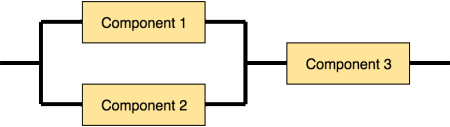
\includegraphics[width=0.5\linewidth]{IndependentEventsExample2.png} \end{center}

    Let $B$ be the event that the signal is blocked. Let $C_1$, $C_2$ and $C_3$ be the events that components $1$, $2$, and $3$ are working. 

    $\begin{aligned}[t]
        P(B) & = P({C_3}^c \cup ({C_1}^c \cap {C_2}^c))                                                     \\
             & = P({C^3}^c) + P({C_1}^c \cap {C_2}^c) - P({C_1}^c \cap {C_2}^c \cap {C_3}^c)                \\
             & = P({C^3}^c) + P({C_1}^c) \times P({C_2}^c) - P({C_1}^c) \times P({C_2}^c) \times P({C_3}^c) \\
             & = 0.01 + 0.1 \times 0.05 - 0.1 \times 0.05 \times 0.01                                       \\
             & = 1.495 \%
    \end{aligned}$
    
    {~~~}

    Alternatively, we can the the indirect method. 

    $\begin{aligned}[t]
        P(B) & = 1 - P(B^c)                                                                                                                    \\
             & = 1 - P(C_3 \cap (C_1 \cup C_2))                                                                                                \\
             & = 1 - P((C_3 \cap C_1) \cup (C_3 \cap C_2))                                                           & \text{distribution law} \\
             & = 1 - \left( P(C_1 \cap C_3) + P(C_2 \cap C_3) - P(C_1 \cap C_2 \cap C_3) \right)                                               \\
             & = 1 - \left( P(C_1) \times P(C_3) + P(C_2) \times P(C_3) - P(C_1) \times P(C_2) \times P(C_3) \right)                           \\
             & = 1 - (0.9 \times 0.99 + 0.95 \times 0.99 - 0.9 \times 0.95 \times 0.99)                                                        \\
             & = 1 - 0.98505                                                                                                                   \\
             & = 1.495 \%
    \end{aligned}$
\end{example}

\section{Bayes' Rule}

Given two events, we know that their conditional probability is defined as $$P(A | B) = \frac{P(A \cap B)}{P(B)} \qquad \text{provided that } P(B) > 0$$ which can be rearranged to $$P(A \cap B) = P(A | B) \cdot P(B)$$

Suppose now we have a sample space consisting \bred{only} of events $A, B_1, B_2, \dots, B_k$ where the $B_i$'s \bred{partitions the sample space}. That is, the $B_i$'s are disjoint and $\bigcup_{i=1}^k B_i = \Omega$. From Axiom 3, we can show that $$P(A) = P(A \cap B_1) + P(A \cap B_2) + \cdots + P(A \cap B_k)$$ Combining this with our knowledge of conditional probability, we get the \bred{Law of Total Probability}.

\begin{theorem}[Law of Total Probability]\index{Law of Total Probability}
    If $B_1, B_2, \dots, B_k$ is a collection of mutually exclusive (disjoint) and exhaustive events that partition the sample space, then for any event $A$, $$P(A) = \sum_{i=1}^n P(A | B_i) \cdot P(B_i)$$
\end{theorem}

Putting together the Law of Total Probability and definition of conditional probability, we get \bred{Bayes' Rule}. 

\begin{theorem}[Bayes' Rule]\index{Bayes' Rule}
    Let $B_1, B_2, \dots, B_k$ form a partition of the sample space and let $A$ be an event in $\Omega$. Than $$\begin{aligned}[t]
        P(B_i | A) & = \frac{P(A \cap B_i)}{P(A)}                                           \\
                   & = \frac{P(A | B_i) \cdot P(B_i)}{\displaystyle \sum_{i=1}^k P(A | B_i) \cdot P(B_i)}
    \end{aligned}$$
\end{theorem}

\begin{example}
    A ball is drawn at random from an urn containing one red and one white ball. If the white ball is drawn, it is put back into the urn. If the red ball is drawn, it is returned to the urn together with two more red balls. Then a second draw is made.

    \begin{enumerate}[label=\alph*)]
        \item What is the probability a red ball was drawn on both the first and the second draws?

        Let $W_i$ be the event where a white ball is drawn on the $i$\textsuperscript{th} draw. 

        Let $R_i$ be the event where a red ball is drawn on the $i$\textsuperscript{th} draw. 

        $\begin{aligned}[t]
            P(R_1 \cap R_2) & = P(R_1) \times P(R_1 | R_1)     \\
                            & = \frac{1}{2} \times \frac{3}{4} \\
                            & = \frac{3}{8}
        \end{aligned}$

        \item What is the probability that a red ball was drawn first if the second ball drawn was red?

        \begin{minipage}[t]{0.35\linewidth}
            \begin{center}
                \tikzsetnextfilename{c03s03-01}
                \begin{tikzpicture}[baseline=(current bounding box.north)]
                    \draw (-1,-1) node {$W_1$};
                    \draw (1,-1) node {$R_1$};
                    %
                    \draw (-1.5,-2) node {$W_2$};
                    \draw (-0.5,-2) node {$R_2$};
                    \draw (0.5,-2) node {$W_2$};
                    \draw (1.5,-2) node {$R_2$};
                    %
                    \draw (0,0) -- (-0.7,-0.7) node[above] {$\sfrac{1}{2}$};
                    \draw (0,0) -- (0.7,-0.7) node[above] {$\sfrac{1}{2}$};
                    %
                    \draw (-1,-1.3) -- (-1.5,-1.7) node[above] {$\sfrac{1}{2}$};
                    \draw (-1,-1.3) -- (-0.5,-1.7) node[above] {$\sfrac{1}{2}$};
                    \draw (1,-1.3) -- (0.5,-1.7) node[above] {$\color{red} \sfrac{1}{4}$};
                    \draw (1,-1.3) -- (1.5,-1.7) node[above] {$\color{red} \sfrac{3}{4}$};
                \end{tikzpicture}
            \end{center}
        \end{minipage}
        \begin{minipage}[t]{0.6\linewidth}
        $\begin{aligned}[t]
            P(R_1 | R_2) & = \frac{P(R_1 \cap R_2)}{P(R_2)}                                                           \\
                         & = \frac{\sfrac{3}{8}}{P(R_1 \cap W_1) + P(R_2 \cap R_1)}                                   \\
                         & = \frac{\sfrac{3}{8}}{P(R_2 | W_1) \times P(W_1) + P(R_2 | R_1) \times P(R_1)}             \\
                         & = \frac{\sfrac{3}{8}}{\sfrac{1}{2} \times \sfrac{1}{2} + \sfrac{3}{4} \times \sfrac{1}{2}} \\
                         & = \frac{3}{5}                                                                              \\
                         & = 60\%
        \end{aligned}$
        \end{minipage}
        
    \end{enumerate}
\end{example}

\begin{example}
    Consider HIV testing. An HIV test will correctly test positive $95\%$ of the time (sensitivity), and incorrectly test positive $1\%$ (false positive rate) of the time. Suppose we know that $99.99\%$ of the population is HIV-free. Under these conditions, what is the probability that a patient who tested positive is actually HIV positive?

    \begin{minipage}[t]{0.4\linewidth}
        \begin{center} 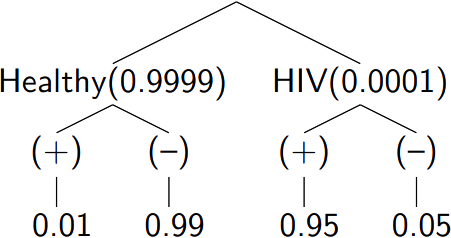
\includegraphics[width=0.75\linewidth,valign=t]{BayesRuleExampleHivTesting.png} \end{center}
    \end{minipage}
    \begin{minipage}[t]{0.55\linewidth}
        $\begin{aligned}[t]
            P(\text{HIV} | +) & = \frac{P(\text{HIV} \cap +)}{P(+)} \\
            & = \frac{P(\text{HIV} \cap +)}{P(+ \cap \text{Healthy}) + P(+ \cap \text{HIV})} \\
            & = \frac{0.95 \times 0.0001}{0.01 \times 0.9999 + 0.95 \times 0.0001} \\
            & = 0.94\%
        \end{aligned}$
    \end{minipage}

    $\therefore$ If we were randomly pick a person and test them for HIV, there chance of them having HIV with a positive test is $0.94\%$. 
\end{example}